%%TO DO: 
%1) Add soft robotics
%3) Add pictures 
%2) A

\chapter{Background}
In this chapter, DWT is positioned with existing technologies. Since DWT is a blend of robotics and wearable electronics, backgrounds for both fields will be provided. Figure~\ref{fig:technologies_size_coverage} summarizes complex relationships between DTW and other technologies. This chapter will look into each technology in the graph in detail, and discuss their advantages and disadvantages. This graph demonstrates the unique and unexplored space that DWT occupies. By looking at the graph, DWT provides variable body coverage while maintaining the size of wearable devices. 


\begin{figure}[!ht]
\centering
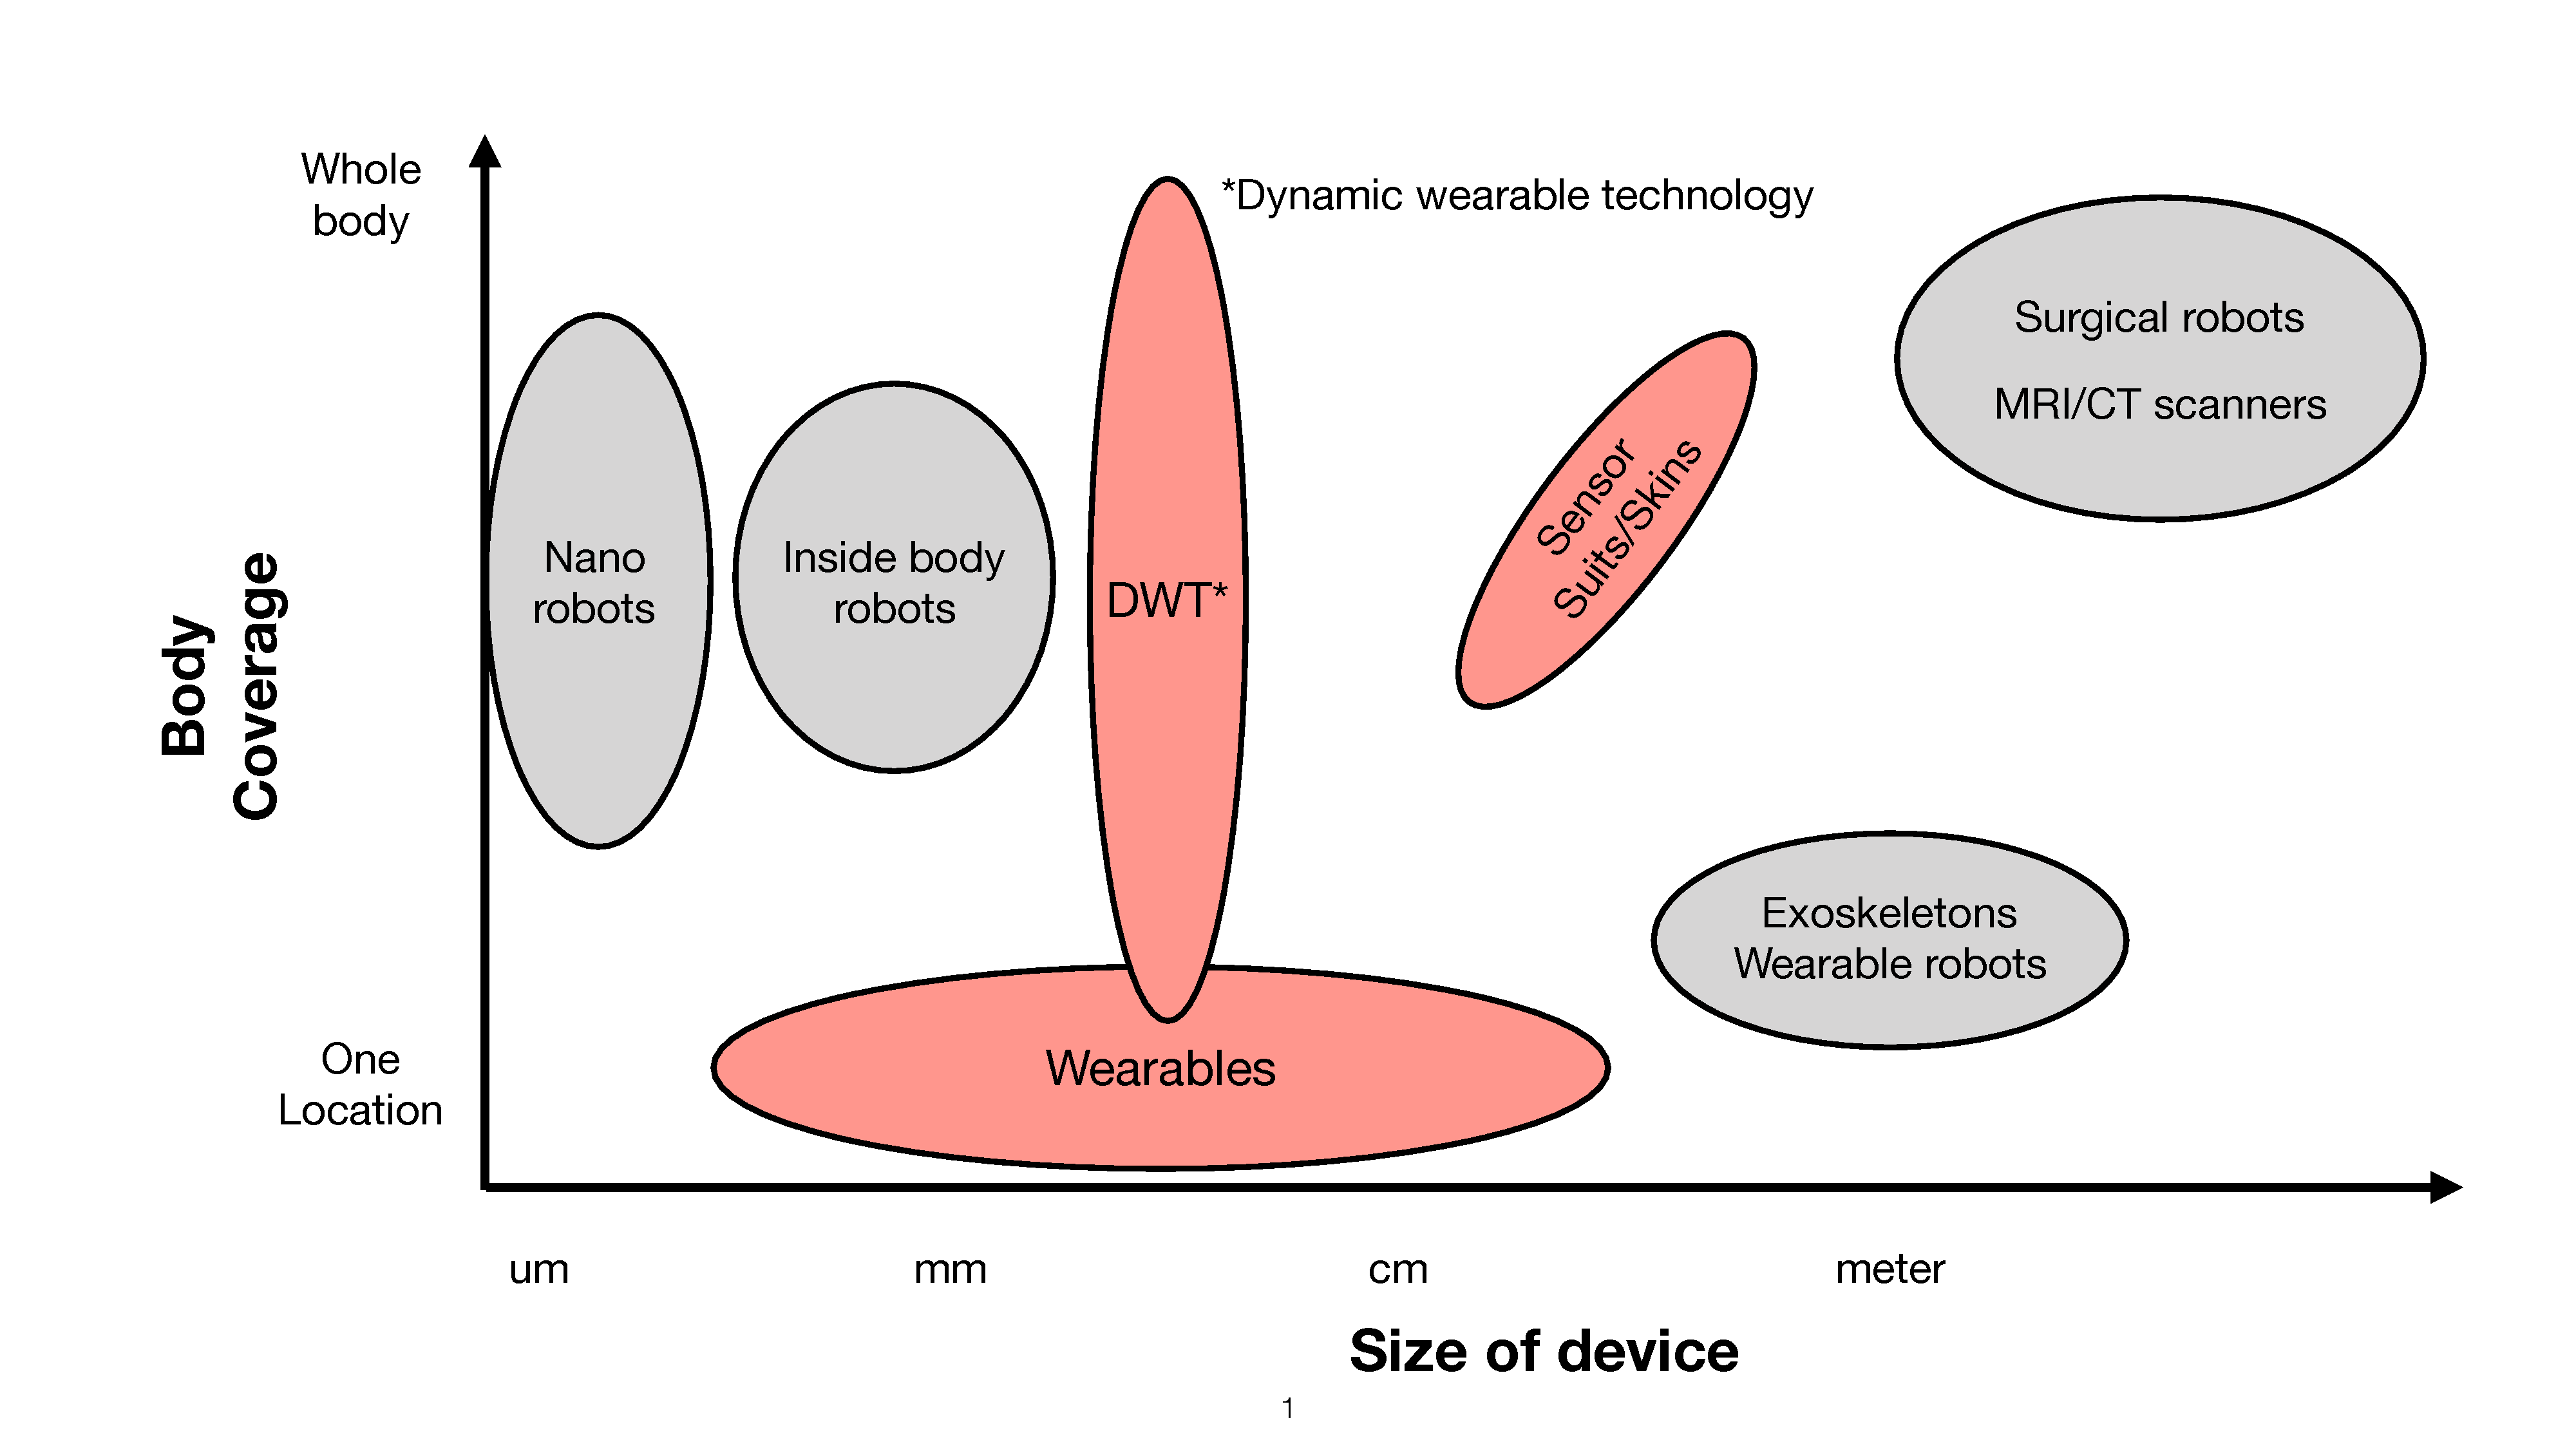
\includegraphics[width=\textwidth]{pictures/chapter2/graph_background.pdf}
\caption{Dynamic wearable technology (DWT) and related technologies. Approximate body coverage of the technology in comparison to it's size. In my previous research and this thesis I explored the technologies highlighted in red.  }
\label{fig:technologies_size_coverage}
\end{figure}

\section{Wearable Electronics}
Wearable first appeared in the early 1960s. The first instance of wearable technology appeared in 1961 as an electric device hidden in the shoe to improve gains at a game of  roulette~\cite{thorp1998invention}. The idea of wearable technology was explored and popularized by Thad Starner and Steve Mann at the MIT Media Lab, with untethered wearable cameras and head-mounted display~\cite{mann1997wearable}. 

Today due to electronics miniaturization, many wearables reached the consumer market. For example, smartwatches are popular. They can provide easily accessible information, as well as sense activity, and limited physiological signals such as heart rate using photoplethysmogram (PPG) with near-infrared spectrometry~\cite{phan2015smartwatch}. Research in Human-Computer Interactions (HCI) has explored many aspects of smartwatches. For example, using motors to provide haptic feedback~\cite{ion2015skin} or to move the watch~\cite{gong2017cito}. Also, researchers explored additional sensing such as electric field~\cite{zhou2016aurasense} on a watch form factor. Today the cutting edge wearable devices research are stretchable tattoo-like epidermal electronics, which has been pioneered by the Rogers group at Urbana Champaign~\cite{kim2011epidermal}. Also, starting with iSkin~\cite{weigel2015iskin}, multiple projects~\cite{lo2016skintillates,kao2016duoskin} in human-computer interactions demonstrated tattoo-like wearables. 

\begin{figure}[!ht]
\centering
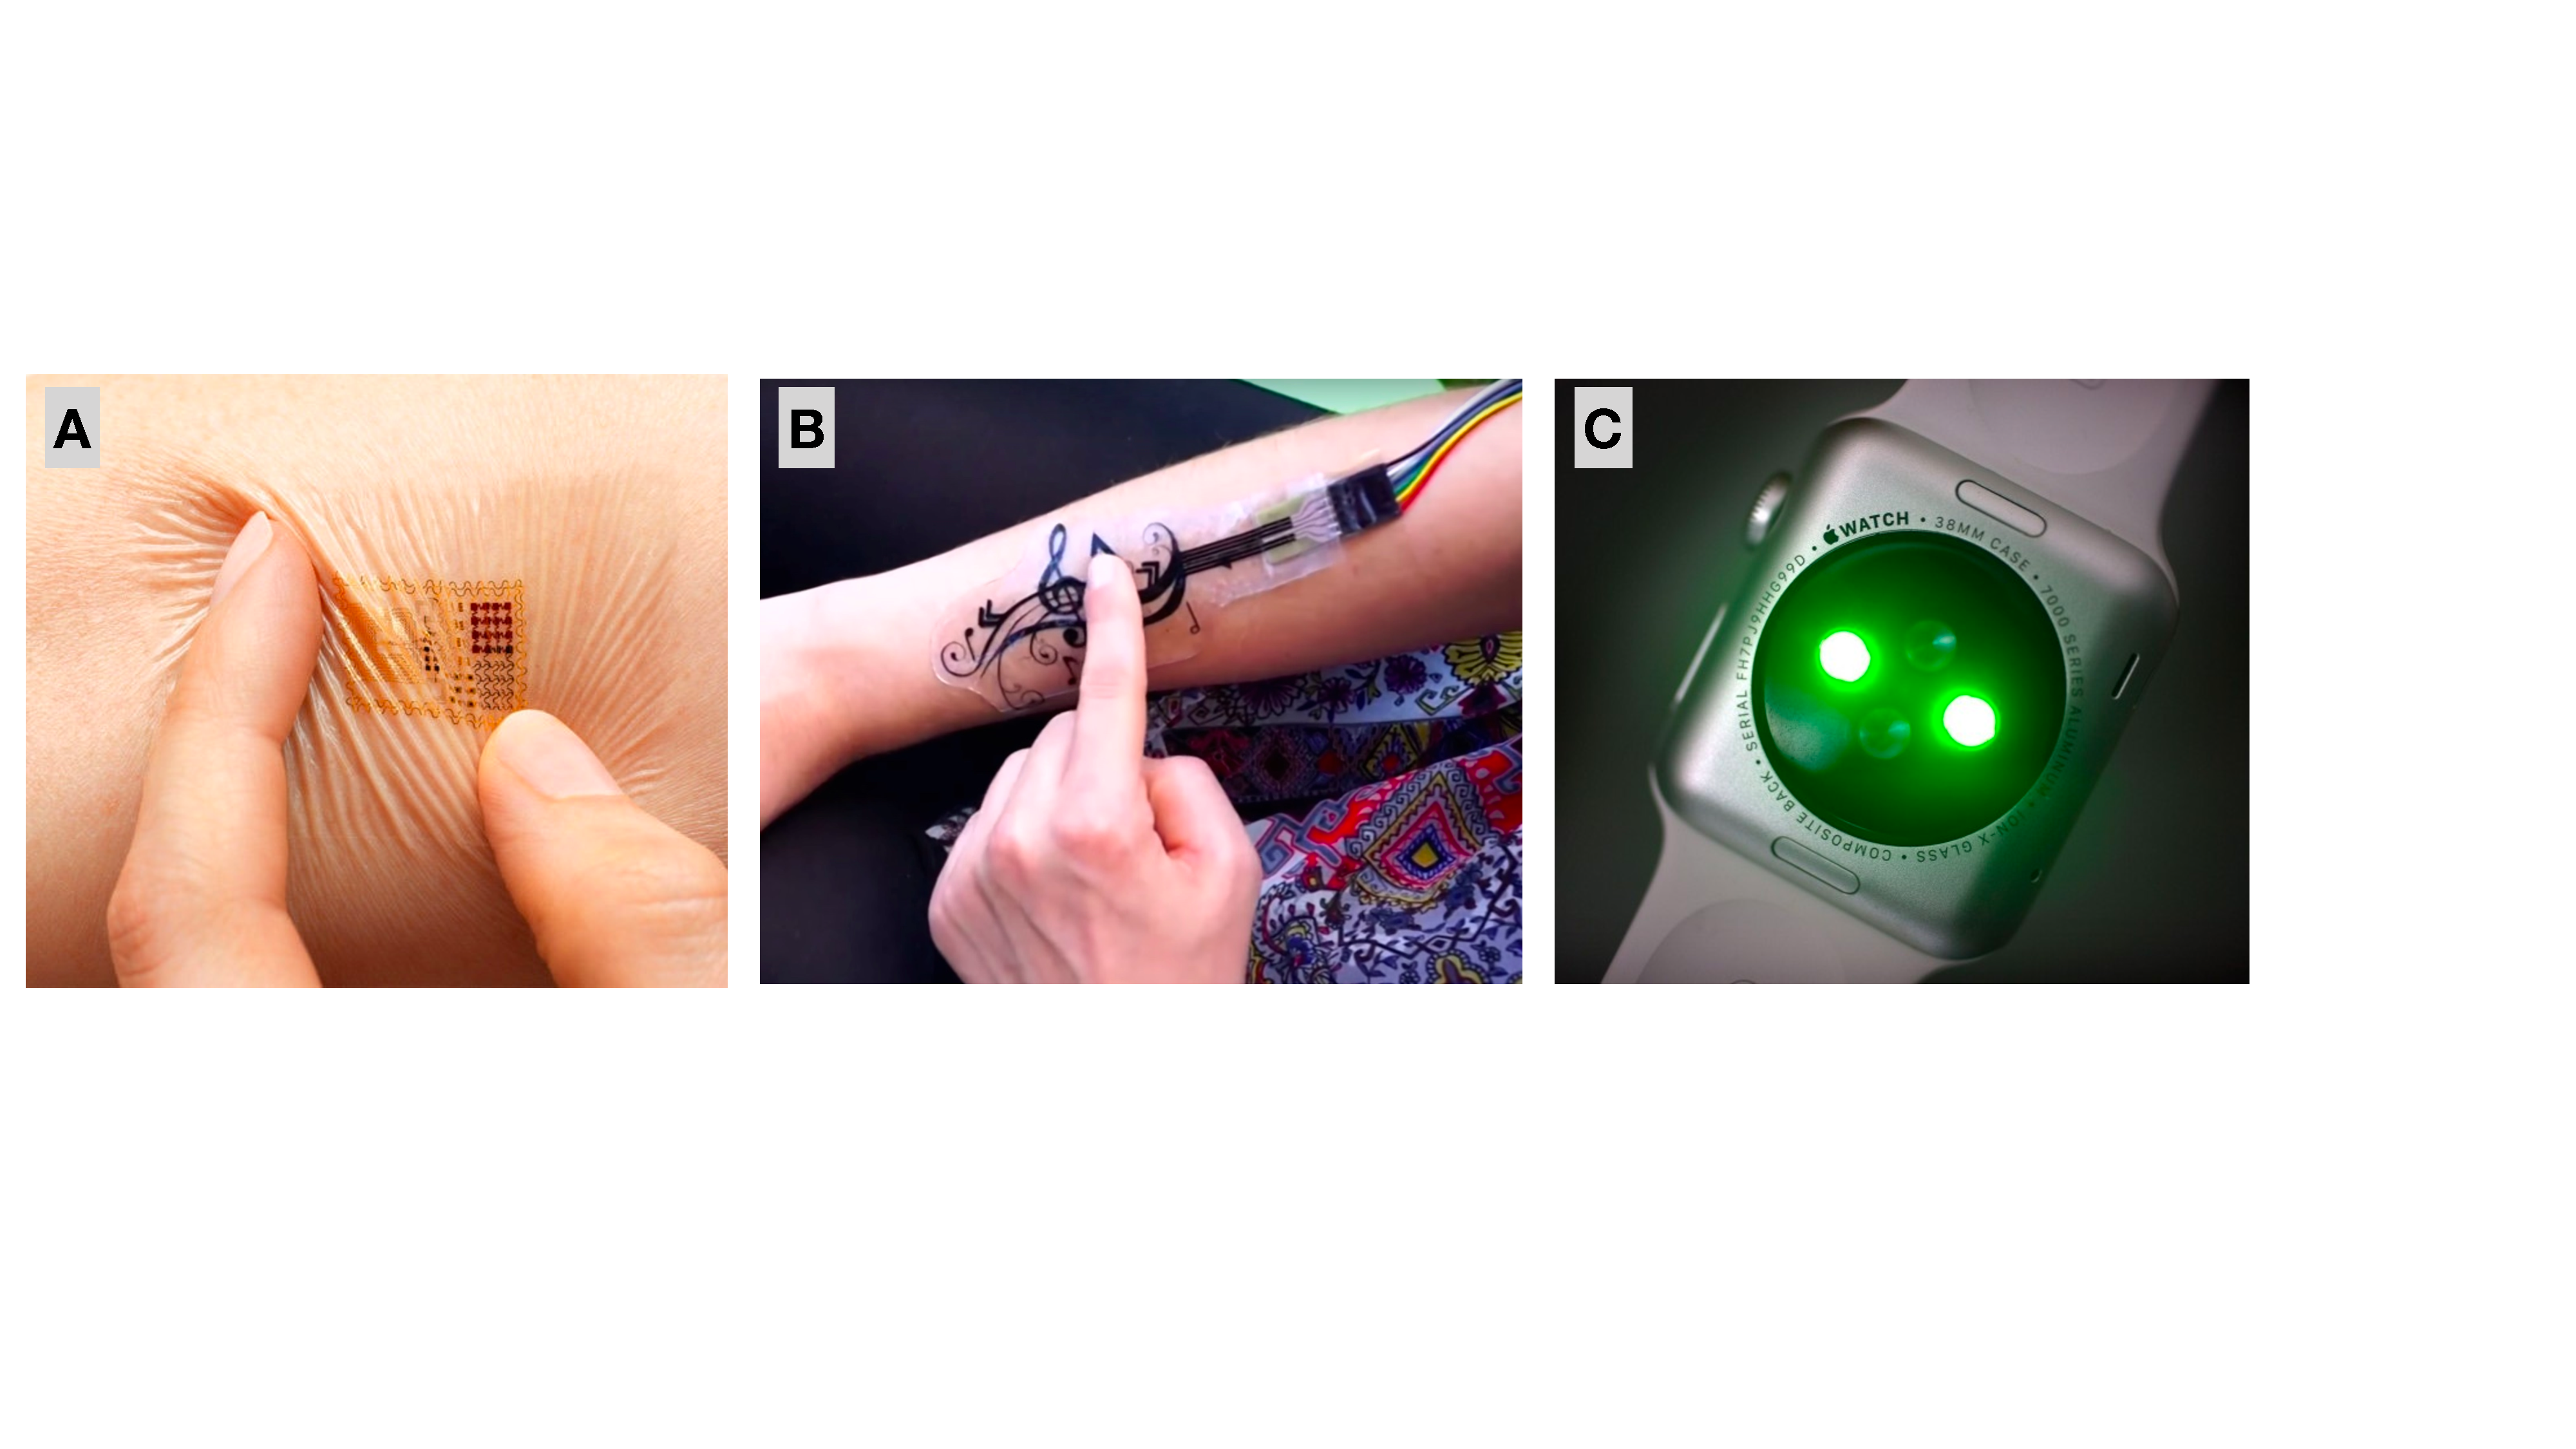
\includegraphics[width=\textwidth]{pictures/chapter2/wearables_basics.pdf}
\caption{Examples of state-of-the-art wearable devices. A) Epidermal electronics: microfabricated stretchable electronics. B) iskin, an on-skin electronics using conductive ink. C) Apple watch with the green LED tuned on, which is used for measuring heartrate and blood oxygen level. }
\label{fig:technologies_size_coverage}
\end{figure}

Wearable devices, including commercial ones and state-of-art research prototypes, are designed to be fixed in one location to perform a specific function. Even though they can vary in size from millimeters to centimeters, wearables cover single point coverage. 

Hovewhere, there are a few exceptions, where researchers and designers looked at moving wearable devices. In a thesis from MIT Media Lab, Zipperbot~\cite{whiton2013sartorial} attaches to a zipper and can zip and unzip clothing.
Other robots did not climb directly on the clothing but demonstrated cloth climbing ideas. The concept of Daily Support Robots~\cite{saga2014daily} showed a robot that moves on the body to provide notifications, using a rail on the arm for climbing. It is one of the earliest examples of moving wearables in Human-Computer Interactions. Movelet is an arm brace that can move up and down, providing haptic feedback~\cite{dobbelstein2018movelet}. 

Fashion designer Hussein Chalayan has done multiple fashion shows with transforming clothing~\cite{transformingClothing}, where motors and pulleys were used to move the dresses. Behnaz Farahi designed a 3D-printed garment that moves based on other people’s gazes~\cite{Graze}. Other designers showed fabrics that can change shape, such as using magnets embedded inside the fabric~\cite{MagneticFabric}. 

\begin{figure}[!ht]
\centering
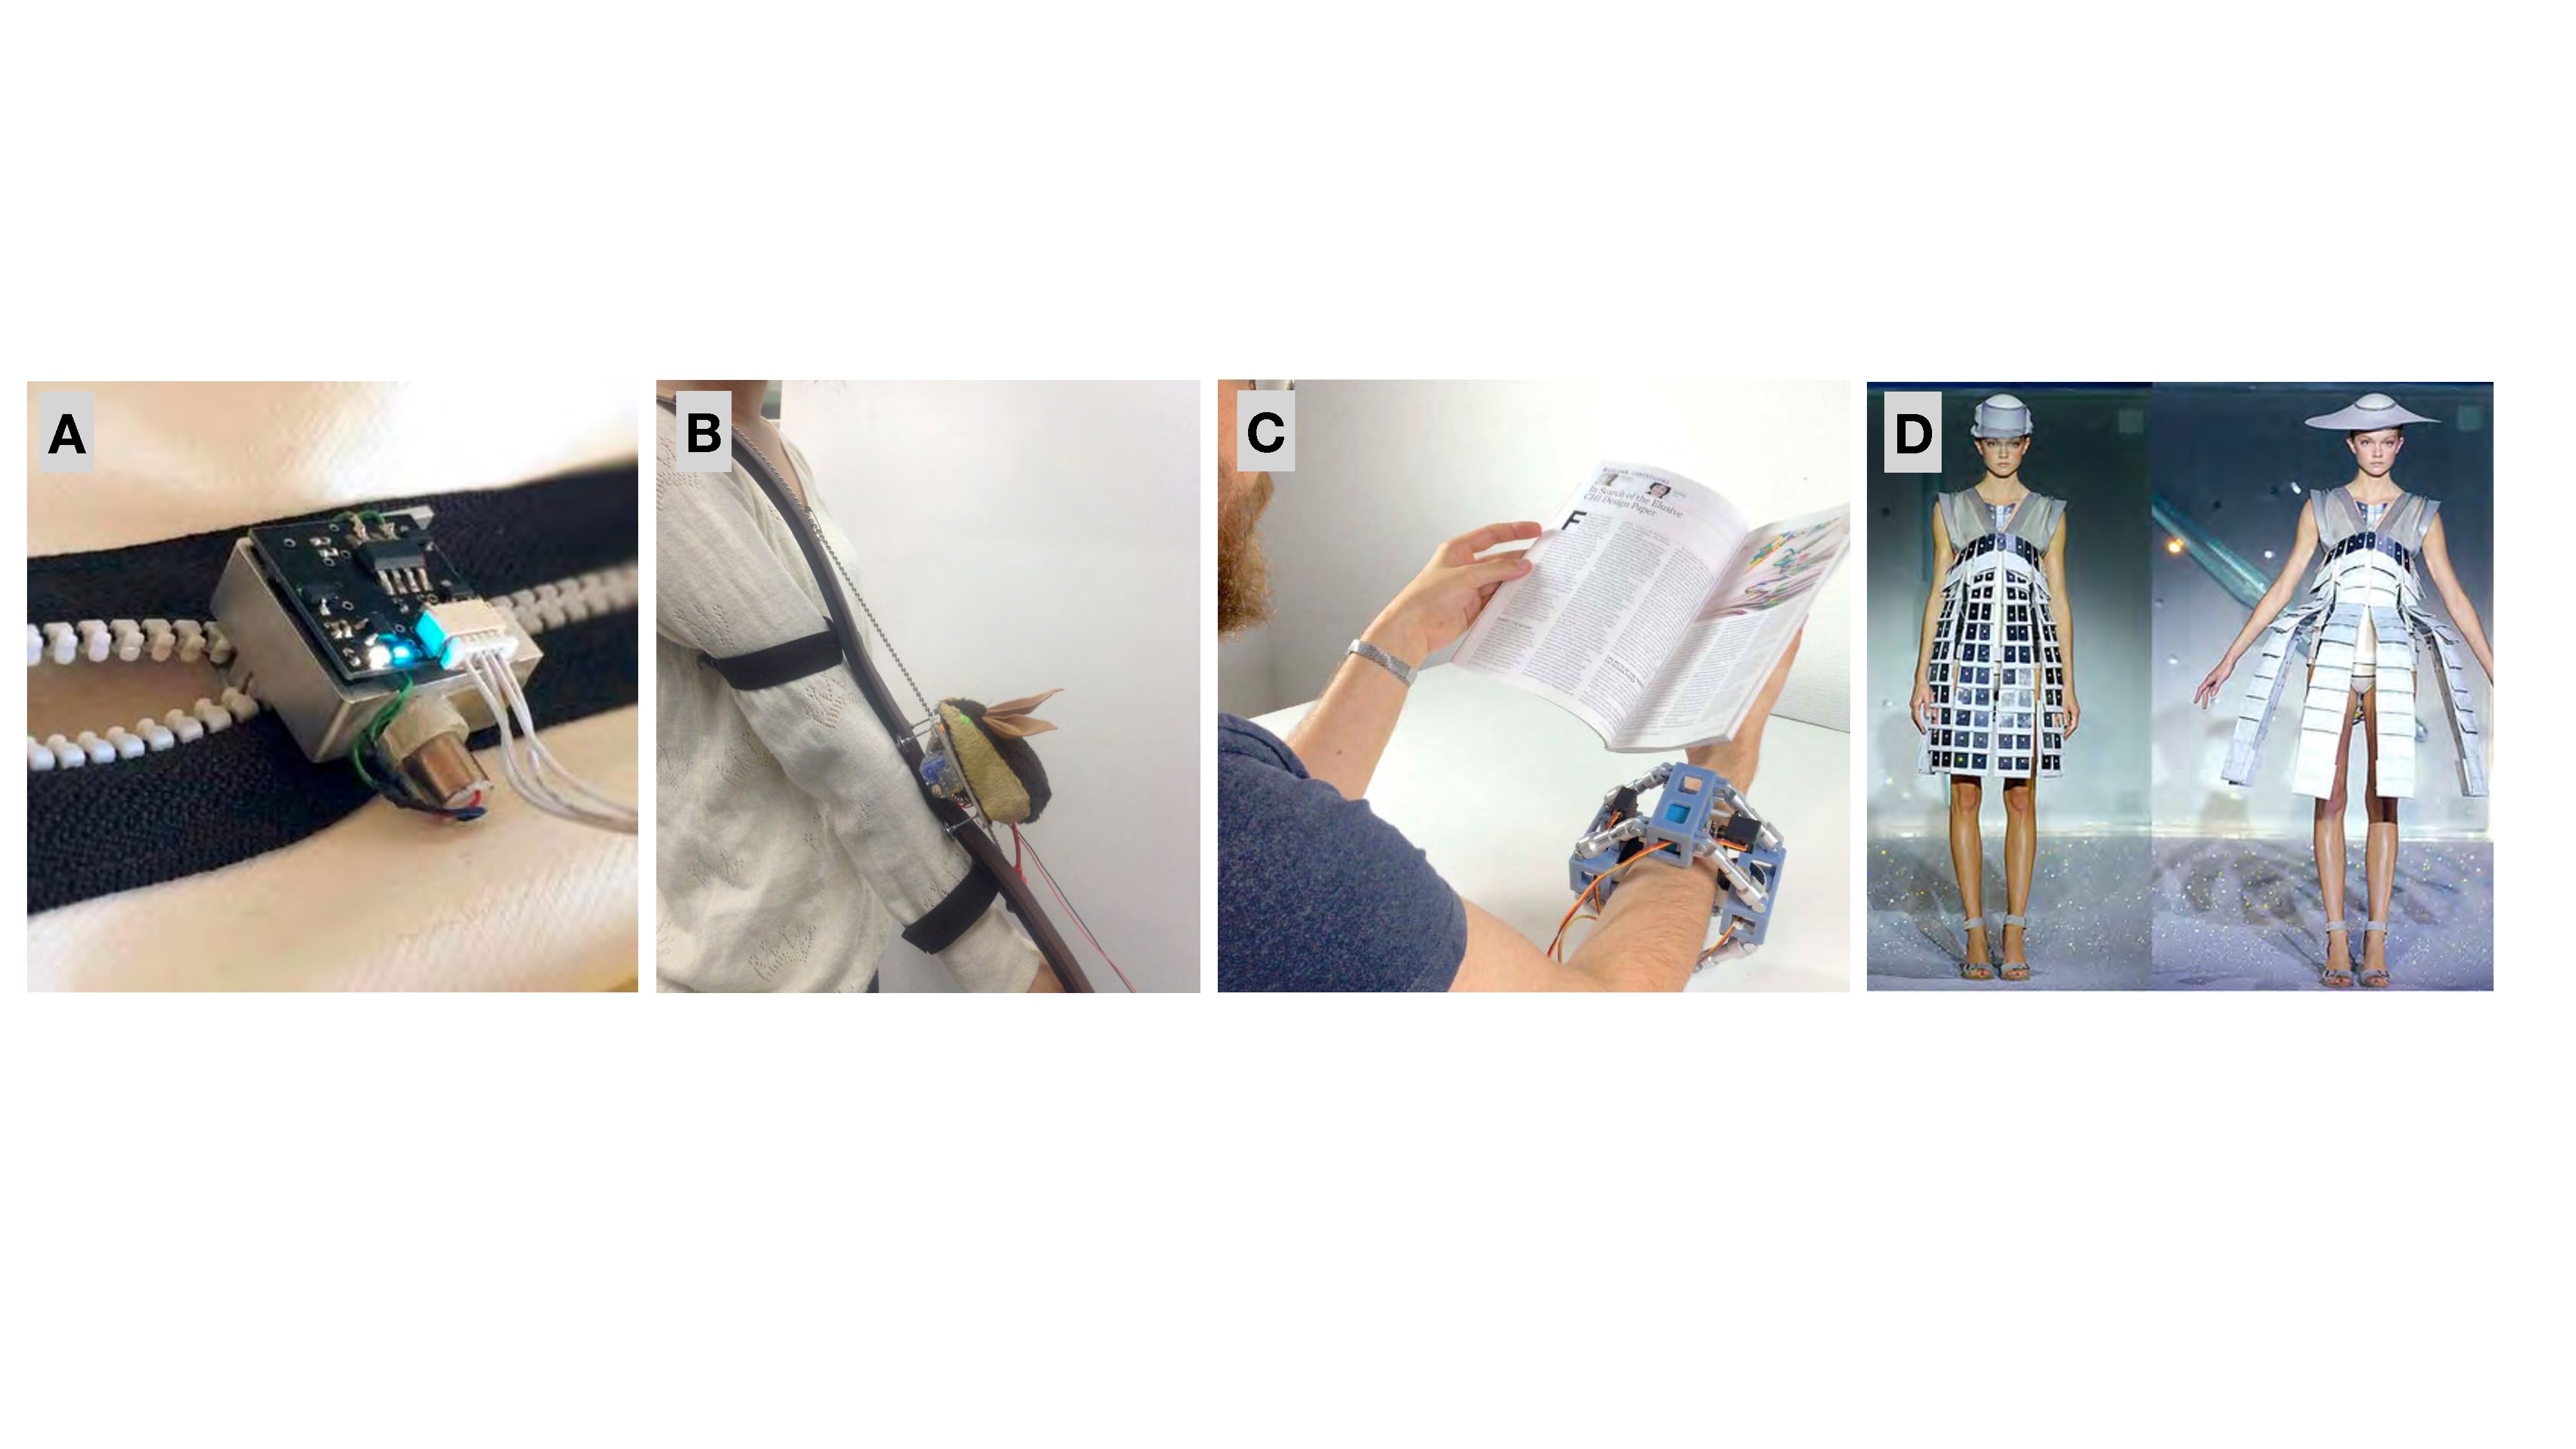
\includegraphics[width=\textwidth]{pictures/chapter2/moving_wearables.pdf}
\caption{Explorations of moving wearable devices and clothing. A) Zipper-bot; a robot that zips clothing. B) Daily support robots, a mouse-looking robot that moves on a rail. C) Movelet, a bracelet that moves up and down the arm for haptic applications. D) Hussein Chalayan fashion show with transforming clothing. }
\label{fig:technologies_size_coverage}
\end{figure}

\section{Sensor fabrics and materials}
A brute force approach is to increase body coverage of sensors is to increase the number of sensors. With this approach, the coverage is directly proportional to the number of sensors. The common approach is using e-textiles,  where electronics are integrated into the fabric. It was first investigated at the MIT Media Lab \cite{post2000broidery} with embroidery of conductive threads. Later was popularized by Leah Buechley with an introduction of LilyPad kit, which made it easier to create e-textiles~\cite{buechley2008lilypad} using friendly form factor and Arduino platform.  This approach has been investigated by Google ATAP recently commercialized jackets with capacitive sensing for gestures~\cite{poupyrev2016project}. A state of the art approach is to integrate semiconductors into textile fibers~\cite{orf2011fiber} directly. Some approaches do not require the sensors to be embedded in the fabric. For example, with 17 inertial measurement units (IMU) placed in pre-defined body locations allows for full 3d body tracking~\cite{roetenberg2009xsens}. In this approach, the suit is used to ensure that the sensors always stay in the same place. 
Another approach is to create flexible sensor skins with various sensors, instead of integrating electronics into the fabrics. For example, Takao Someya's group at the University of Tokyo demonstrated a flexible pressure sensor array for robotic applications~\cite{someya2004large}.
As a precedent to DWT, we demonstrated  SensorTape. It could be used as a wearable sensor skin to track posture as well as be cut to different sizes~\cite{dementyev2015sensortape}. 

There are multiple disadvantages to using sensor materials. First, it requires custom fitting fabrics to ensure good contact with the skin. Second, there is a scaling problem with an increasing number of sensors. The size, complexity, price, and power consumption increases with the coverage. It is not an issue for simple sensors such as electrodes, but a problem with multiple sensors such as cameras. Nevertheless, this approach is promising. With the improvements in electronics size and power, we can integrate more and more sensors in clothing. 

\begin{figure}[!ht]
\centering
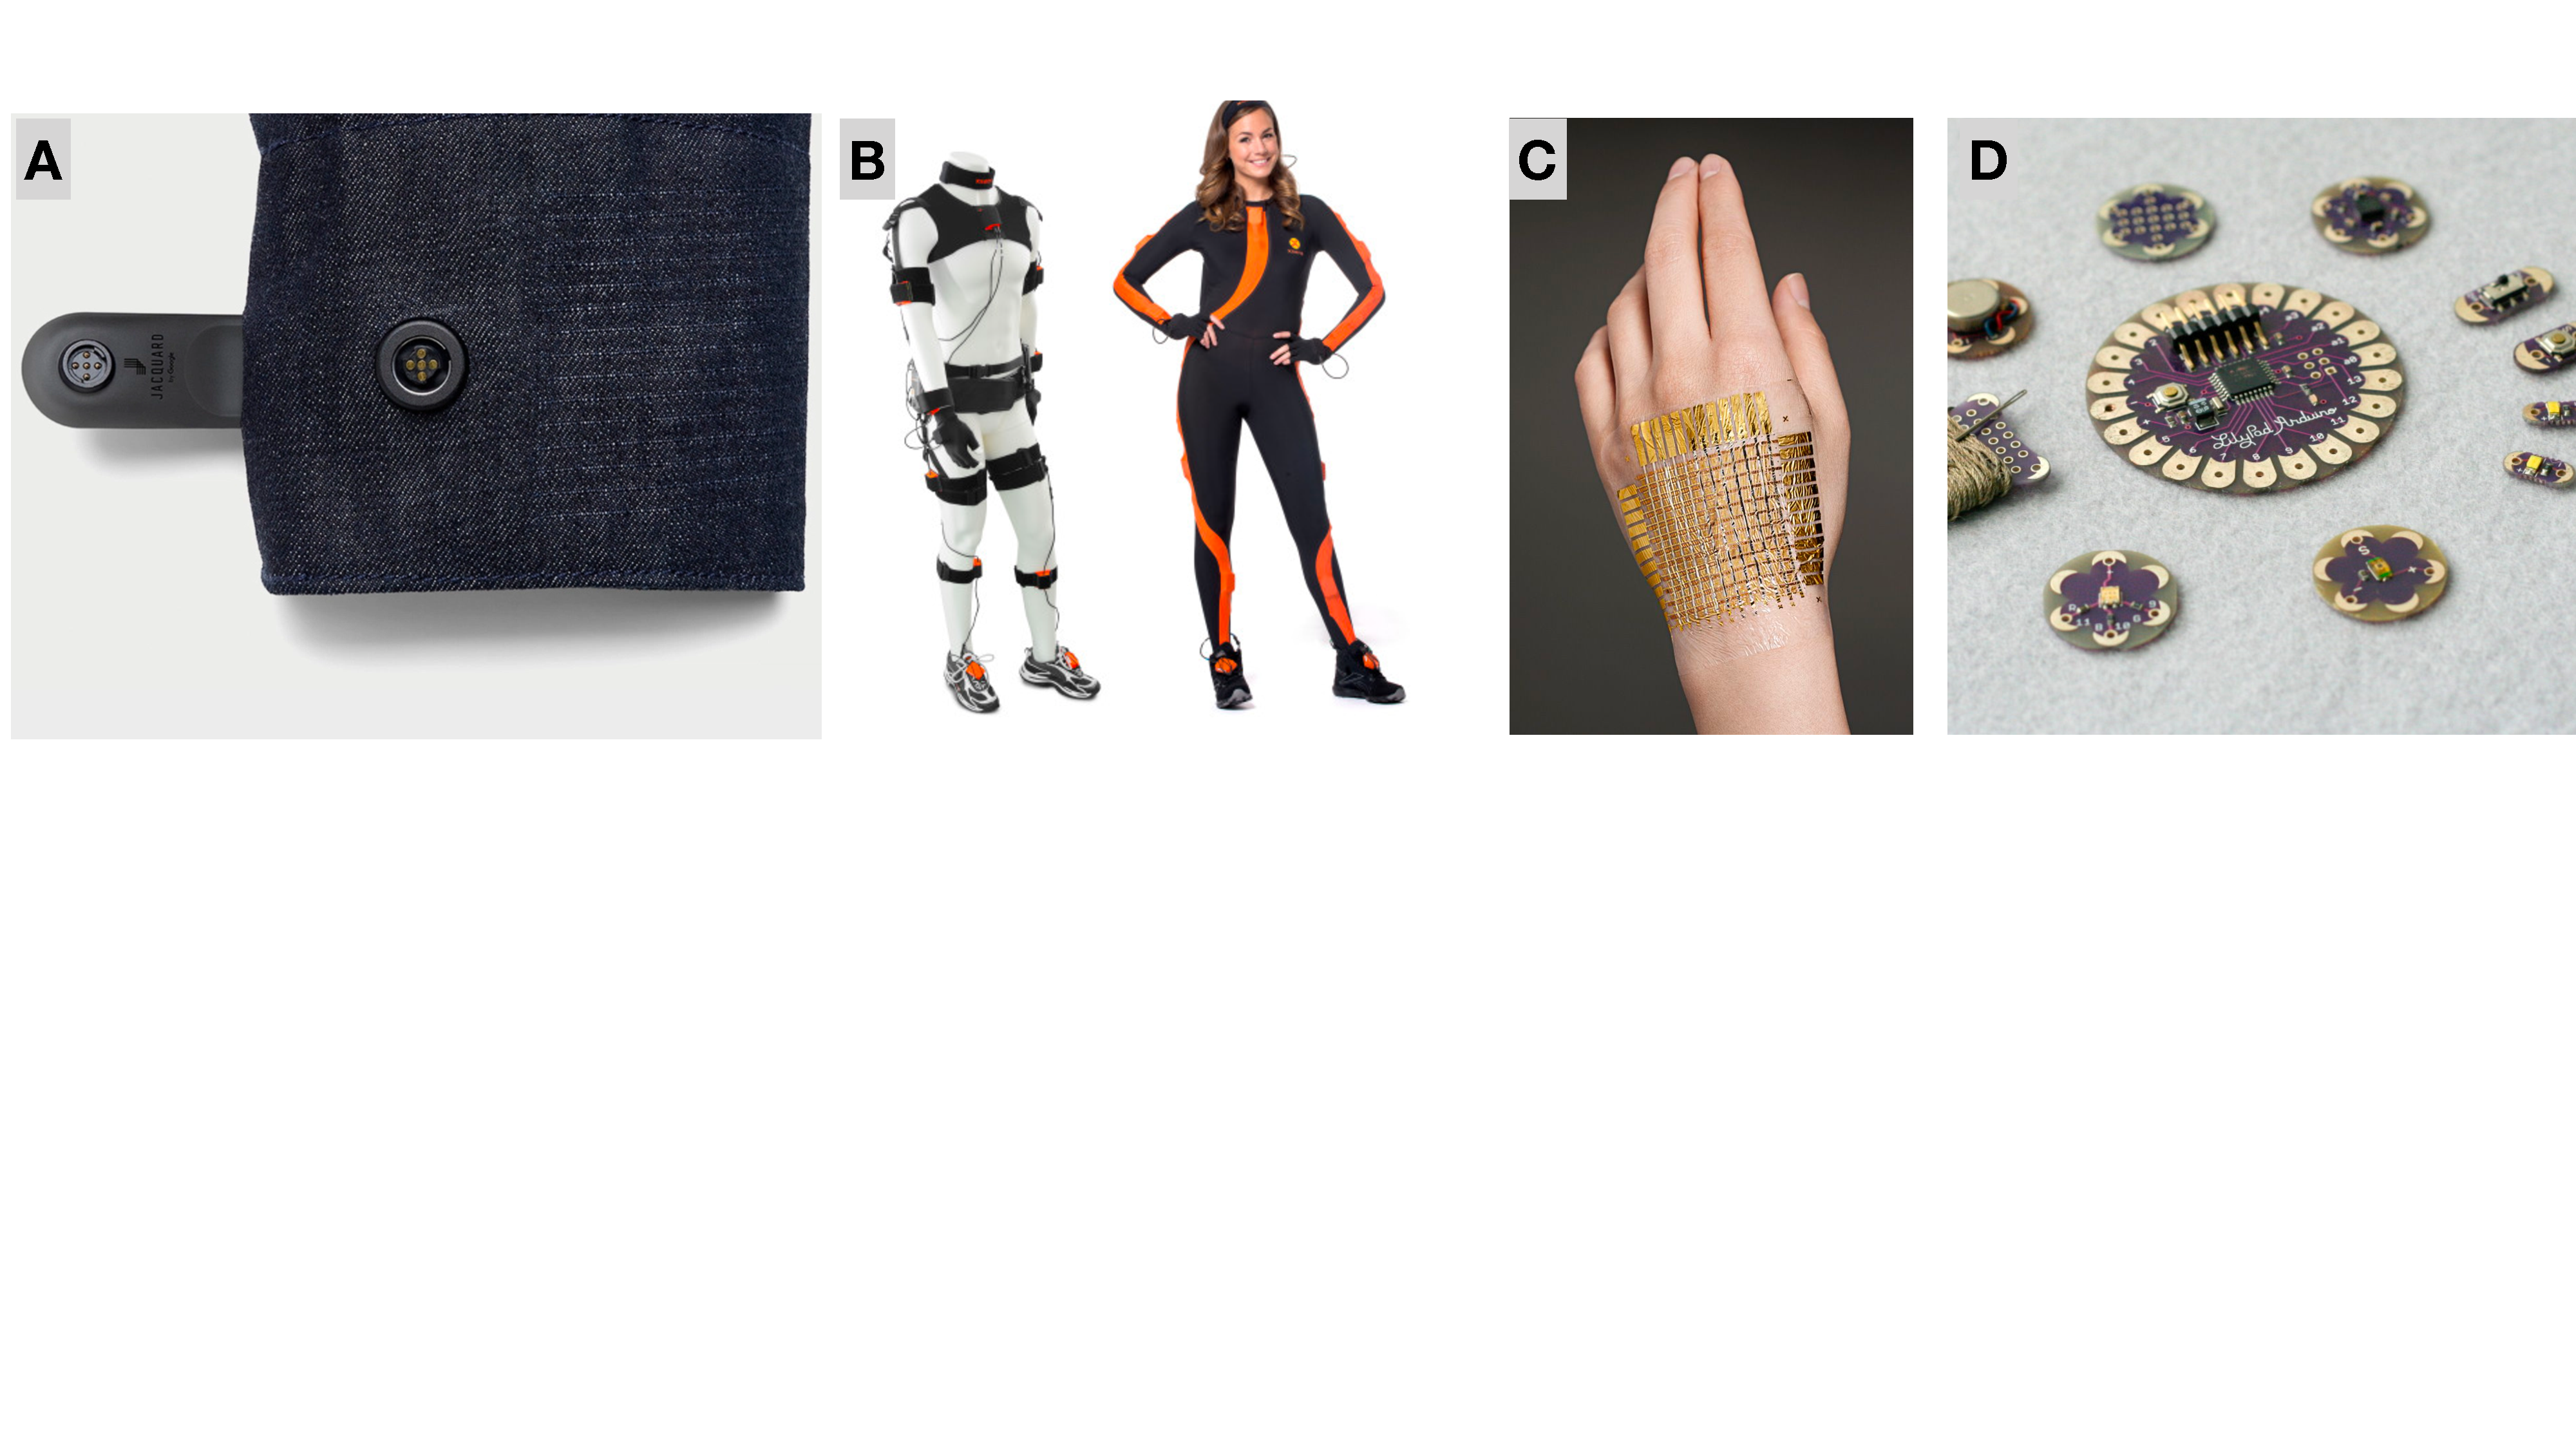
\includegraphics[width=\textwidth]{pictures/chapter2/textiles_sensors.pdf}
\caption{Examples of sensor suits and skins. A) Denum Jacket with capactive sensing conductive fibers. B) Body motion capture suit from Xsens. C) Pressure sensor skin from Takao Someya's group. D) LillyPad Arduino, a kit for wearable electronics. }
\label{fig:technologies_size_coverage}
\end{figure}


\section{Micro and nano robots}
Nanorobots and microrobots that go inside the body is an area of active research. The advantage of the microrobots is that they can be non-invasively injected into the body. There are significant challenges to realizing this, such as power and size, so off-the-shelf technology cannot be used. There were robots proposed to move inside blood vessels~\cite{cavalcanti2006nanorobot}. Many microrobots are steered by external magnetic fields ~\cite{nelson2010microrobots}. Some exciting work has focused on how a swarm of robots can be inserted through a needle and assembled inside the eye~\cite{wu2018swarm}. Some robots were actuated by shape memory alloy wires~\cite{webster2006toward}. 

 The main disadvantage of mini/nanorobots is their limited functionality. It is not yet technically possible to integrate computing and energy sources into such robots, so they lack autonomy. Usually, they are driven by an external machine, so the person remains tethered to a specific location.

\section{Mini-robots inside the body}
 The mini-robots also go inside the human body but are larger than the nano and microrobots. They are usually on millimeter to centimeter scale. They can potentially be autonomous, as they can contain computing and power source. There are task-specific medical prototype robots such as small bone mounting robot for spine surgery~\cite{shoham2003bone}, a snake-like robot that goes into the airways~\cite{simaan2004high}, and an endoscope robot to look inside the body cavities~\cite{yoon2011active}. Most relevant to DWT is HeartLander~\cite{patronik2005preliminary,patronik2004crawling}, Carnegie Mellon's robot that uses suction to locomote on the surface of the heart and deliver injections. The robot has been tested on a beating pig heart. The robot was developed in the early to mid-2000s and appeared to be in the commercialization stage.
 
 The disadvantage of mini robots is that they are invasive. The robots are too large, so they require an invasive entry into the body. DWT is on the same size scale, but it is not invasive. 

\section{Room-size devices}
Full body coverage can be achieved by putting the person inside a large machine or having a large robot. Typically, a large machine such as a CT or MRI scanner is used. 
Another approach is using non-contact sensing, such as radio signals~\cite{adib2015smart} or cameras~\cite{mcduff2014improvements} to sense heart rate and respiration. 

Some surgical robots are already being used in medicine. Those are large robots that can perform surgery with teleoperation. There are two main such robots: the research robot Raven~\cite{rosen2011raven} and commercial Da Vinci robot~\cite{tewari2002technique}.

The main disadvantage of large machines is that the person requires to be enclosed by the device or remain in a specific location, so this approach can not be used in an ambulatory setting. 

\section{Exoskeletons}
Currently, the term wearable robots refer to exoskeletons. 
Exoskeleton's role is to improve or substitute human abilities. Some can be purely medical, such as an active prosthesis. For example, an artificial hand controlled by EMG signals~\cite{bitzer2006learning}. The applications of such robots are straightforward: to restore the function of a missing or damaged limb. The second application of exoskeletons is to improve abilities or to add haptics. For example, an upper arm exoskeleton was developed by Columbia University~\cite{perry2007upper}. Other researcher made additional appendages such as fingers~\cite{leigh2016body}.

% point of this section? 

\section{Summary}
In this section, various technologies regarding body coverage and size were presented. There are advantages and disadvantages to each technology. DWT occupies a unique niche in the space. 
% Could be in the other section 


%\section{Robots in different fields}
%\subsection{Robots in Medicine}
%There are two main categories of medical robots: outside the body and inside the body. Currently, there are no works with moving robots on the body for medical applications. In terms of size, the on-body robots are on a scale that hasn’t been explored. Usually, research focuses on big things (regular robots) or tiny things (nano). Most of the medical robots now are large stationary machines or attached to a specific location of the body, (e.g., prosthesis). 